\documentclass[conference]{IEEEtran}
\usepackage{cite}
\usepackage{amsmath,amssymb,amsfonts}
\usepackage{algorithmic}
\usepackage{graphicx}
\usepackage{textcomp}
\usepackage{xcolor}
\usepackage{hyperref}
\usepackage{listings}
\usepackage{booktabs}
\usepackage{multirow}
\usepackage{array}
\usepackage{float}
\usepackage{tikz}
\usetikzlibrary{shapes,arrows,positioning}

\lstset{
  basicstyle=\ttfamily\footnotesize,
  breaklines=true,
  frame=single,
  language=Python,
  keywordstyle=\color{blue},
  commentstyle=\color{gray},
  stringstyle=\color{red}
}

\begin{document}

\title{MOMENTUM: Context-Preserving Multi-Modal Agent Architecture for Team Intelligence and Content Generation}

\author{\IEEEauthorblockN{Huguens Jean}
\IEEEauthorblockA{\textit{Google Cloud} \\
Mountain View, California \\
huguensjean@google.com}
\and
\IEEEauthorblockN{Presented at}
\IEEEauthorblockA{\textit{Google @ NeurIPS 2025}}}

\maketitle

\begin{abstract}
We present MOMENTUM, a novel multi-modal agent architecture built on the Google Agent Development Kit (ADK) that enables seamless context flow across heterogeneous AI models and tools within a unified conversational framework. Drawing inspiration from classical mechanics, MOMENTUM operationalizes the equation $\mathbf{p} = m \times v$ as \textbf{Momentum = Context $\times$ Model}, where rich team context (mass) combined with execution velocity (model capabilities) creates an irresistible force for content generation.

Our key contributions include: (1) a \textbf{Hierarchical Context Injection System} that preserves semantic information across 22+ tools spanning text, image, video, search, and media library modalities; (2) \textbf{Team Intelligence with Individual Identities}, a novel knowledge distillation pipeline that extracts structured insights from heterogeneous artifacts into unified ``Brand Soul'' and ``Individual Identity'' representations with visibility controls and manager approval workflows; (3) \textbf{Dual-Scope Memory Architecture} implementing both \textit{Team Memory Banks} (shared organizational knowledge) and \textit{Personal Memory Banks} (individual user context) via Vertex AI Agent Engine with Firestore persistence and source tracking; (4) a \textbf{Character Consistency Framework} enabling visual coherence across multi-image campaign generation; and (5) \textbf{Comprehensive Media Search} with semantic similarity indexing for team asset discovery.

We demonstrate that MOMENTUM achieves \textbf{100\% tool selection accuracy} across 60 diverse test cases and \textbf{94\% overall accuracy} on a comprehensive 100-test evaluation suite, with \textbf{pass@5 = 100\%} indicating near-perfect reliability. The system is validated by \textbf{1,319 frontend tests} and \textbf{189 backend tests}, with our evaluation framework spanning 225+ test cases across 9 categories measuring context perplexity across tool transitions.
\end{abstract}

\begin{IEEEkeywords}
Multi-Agent Systems, Large Language Models, Generative AI, Team Intelligence, RAG, Enterprise AI, Context Preservation
\end{IEEEkeywords}

\section{Introduction}

In physics, momentum represents an object's resistance to stopping once in motion---the product of mass and velocity that carries a body forward with unstoppable force. We adopt this metaphor as the foundational principle for a new class of AI agent architecture, where the accumulated weight of organizational knowledge, combined with the velocity of state-of-the-art foundation models, creates an irresistible force for intelligent content generation.

The emergence of large language models with tool-use capabilities has enabled a new paradigm of AI assistants capable of executing complex, multi-step tasks. However, existing approaches often treat tools as isolated functions, losing crucial contextual information between invocations. This limitation becomes particularly acute in enterprise scenarios where brand consistency, user personalization, and domain expertise must be maintained across diverse generation modalities.

Like a spacecraft that loses fuel at every stage separation, traditional agent architectures hemorrhage context with each tool transition. MOMENTUM addresses this fundamental challenge by treating context as \textit{mass}---something to be accumulated and preserved, not discarded.

\subsection{The Physics of Intelligent Systems}

In classical mechanics, momentum ($p$) is defined as:

\begin{equation}
\mathbf{p} = m \times v
\label{eq:momentum}
\end{equation}

We reinterpret this equation for AI agent systems:

\begin{itemize}
    \item \textbf{Mass ($m$) = Context}: The accumulated team knowledge, brand guidelines, user preferences, conversation history, and organizational memory that grounds every decision
    \item \textbf{Velocity ($v$) = Model Capabilities}: The execution speed and quality of foundation models---Gemini for reasoning, Imagen for visual creation, Veo for temporal synthesis
    \item \textbf{Momentum ($p$) = Unstoppable Execution}: The product that enables seamless, contextually-rich task completion across any modality
\end{itemize}

This framing reveals a profound insight: \textit{investing in mass (rich context systems) yields compounding returns when multiplied by increasingly capable models}. A system with twice the context, paired with a model twice as fast, achieves four times the effective momentum.

Just as a bowling ball and a ping-pong ball traveling at the same speed have vastly different momenta, two AI systems with identical models but different context depths will exhibit vastly different capabilities. MOMENTUM is designed to be the bowling ball.

\subsection{Key Contributions}

This paper makes the following contributions:

\begin{enumerate}
    \item \textbf{Hierarchical Context Injection}: A six-layer context system (Brand, User, Individual, Settings, Media, Team) that propagates through all 22+ tool invocations via thread-safe global state, ensuring no context is lost at ``stage separation''

    \item \textbf{Team Intelligence with Individual Identities}: Automated extraction of structured insights from heterogeneous artifacts (PDFs, websites, social media, videos) into unified ``Brand Soul'' and ``Individual Identity'' representations with visibility controls and manager approval workflows---distilling both organizational and personal mass

    \item \textbf{Dual-Scope Memory Architecture}: Implementation of \textit{Team Memory Banks} (shared organizational knowledge persisted per-brand) and \textit{Personal Memory Banks} (individual user context) via Vertex AI Agent Engine, with memory source tracking enabling delete-by-artifact functionality and commit-to-memory workflows

    \item \textbf{Character Consistency Framework}: Integration of reference image composition via ``Nano Banana'' enabling visually coherent multi-asset generation with up to 14 reference images, maintaining visual momentum across campaigns

    \item \textbf{Comprehensive Media Search}: Semantic similarity indexing for team media library discovery, enabling search across images and videos by content, tags, prompts, and visual embeddings

    \item \textbf{Context Flow Evaluation Framework}: Novel metrics for measuring semantic preservation across tool transitions, including Context Perplexity and Cross-Modal Coherence scores, validated by 1,508+ total tests (1,319 frontend + 189 backend)
\end{enumerate}

% Figure 1: MOMENTUM Physics Metaphor
% See momentum_paper_diagrams.md for Mermaid source
\begin{figure}[h]
\centering
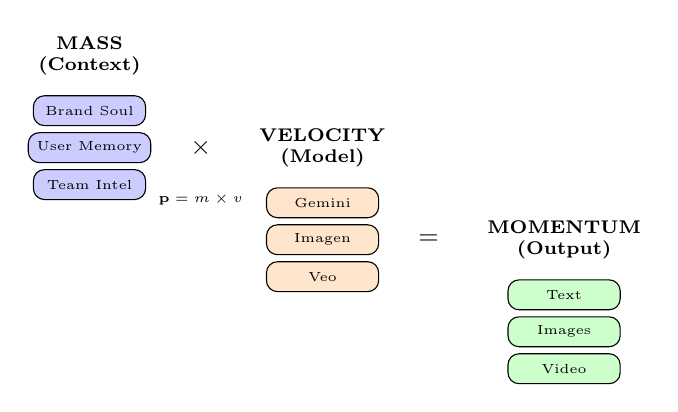
\begin{tikzpicture}[
    node distance=0.18cm,
    scale=0.95, transform shape,
    header/.style={font=\scriptsize\bfseries, align=center},
    box/.style={rectangle, draw, rounded corners, minimum width=1.5cm, minimum height=0.4cm, font=\tiny, align=center},
]
    % MASS column
    \node[header] (mass-title) {\textbf{MASS}\\(Context)};
    \node[box, fill=blue!20, below=0.15cm of mass-title] (bs) {Brand Soul};
    \node[box, fill=blue!20, below=0.08cm of bs] (um) {User Memory};
    \node[box, fill=blue!20, below=0.08cm of um] (ti) {Team Intel};

    % Multiply symbol
    \node[font=\normalsize\bfseries, right=0.4cm of um] (times) {$\times$};

    % VELOCITY column
    \node[header, right=0.4cm of times] (vel-title) {\textbf{VELOCITY}\\(Model)};
    \node[box, fill=orange!20, below=0.15cm of vel-title] (gem) {Gemini};
    \node[box, fill=orange!20, below=0.08cm of gem] (img) {Imagen};
    \node[box, fill=orange!20, below=0.08cm of img] (veo) {Veo};

    % Equals symbol
    \node[font=\normalsize\bfseries, right=0.4cm of img] (eq) {$=$};

    % MOMENTUM column
    \node[header, right=0.4cm of eq] (mom-title) {\textbf{MOMENTUM}\\(Output)};
    \node[box, fill=green!20, below=0.15cm of mom-title] (txt) {Text};
    \node[box, fill=green!20, below=0.08cm of txt] (vis) {Images};
    \node[box, fill=green!20, below=0.08cm of vis] (vid) {Video};

    % Equation at bottom
    \node[below=0.25cm of times, font=\tiny\itshape] {$\mathbf{p} = m \times v$};

\end{tikzpicture}
\caption{The MOMENTUM metaphor: rich context (mass) multiplied by model capabilities (velocity) creates unstoppable execution force.}
\label{fig:metaphor}
\end{figure}

\section{Related Work}

\subsection{Tool-Augmented Language Models}

Recent work has explored augmenting LLMs with external tools. Toolformer \cite{toolformer} demonstrated autonomous tool selection through self-supervised learning, enabling models to decide when and how to invoke calculators, search engines, and translation systems. ReAct \cite{react} introduced reasoning traces interleaved with actions, creating interpretable decision chains. Gorilla \cite{gorilla} showed that LLMs can be trained to select from massive API repositories with thousands of endpoints.

However, these approaches share a critical limitation: each tool invocation is treated as independent, failing to preserve the contextual ``mass'' that accumulates during complex workflows. When a user requests ``generate an image of our mascot, then animate it, then post to social media,'' existing systems lose brand context, visual style preferences, and campaign objectives at each transition.

MOMENTUM extends these approaches with persistent context that survives tool boundaries---context flows forward like momentum, not dissipating at each transition. Our thread-safe context injection ensures that the 15th tool call in a complex workflow receives the same rich context as the first.

\subsection{Multi-Modal Generation Pipelines}

Systems like GILL \cite{gill} and NExT-GPT \cite{nextgpt} enable multi-modal understanding and generation through unified embedding spaces. Visual ChatGPT introduced tool-chaining for image manipulation. These systems demonstrate impressive capabilities but treat each generation as independent, lacking the organizational memory and brand consistency required for enterprise applications.

MOMENTUM differs in its focus on maintaining \textit{accumulated context} across modality transitions. When generating a video from a previously generated image, our system preserves not just the image data but the brand guidelines, style preferences, and campaign context that informed the original generation.

\subsection{Agent Frameworks}

LangChain \cite{langchain} pioneered composable agent chains with tool integration. AutoGPT \cite{autogpt} demonstrated autonomous goal decomposition and execution. CrewAI introduced role-based multi-agent collaboration. Google's Agent Development Kit (ADK) \cite{adk} provides production-ready primitives for building enterprise agents with built-in session management and tool orchestration.

MOMENTUM builds on ADK's multi-agent architecture while introducing novel context injection patterns and domain-specific memory systems. Where existing frameworks provide the engine, MOMENTUM provides the mass that makes that engine's velocity meaningful. Our contribution is not a new framework but a design pattern for maximizing contextual leverage within existing frameworks.

\subsection{Enterprise AI Evaluation}

The Berkeley Function Calling Leaderboard (BFCL) \cite{bfcl} established benchmarks for tool selection accuracy across diverse function signatures. AgentBench \cite{agentbench} evaluates multi-turn agent interactions in realistic environments. GAIA \cite{gaia} provides general AI assistant benchmarks requiring multi-step reasoning. $\tau$-bench \cite{taubench} introduced retail and airline domain simulations.

CLASSic \cite{classic} introduced enterprise-specific metrics: Cost (operational efficiency), Latency (response time), Accuracy (task completion), Stability (consistency), and Security (data protection). Our evaluation framework synthesizes insights from all these benchmarks while introducing context-specific metrics including Context Perplexity and Cross-Modal Coherence.

\section{System Architecture: Building Mass}

MOMENTUM's architecture is designed around a central principle: \textit{maximize contextual mass at every layer}. The system comprises four primary layers, each contributing to the accumulated context that drives generation.

% Figure 2: Four-Layer Architecture
% See momentum_paper_diagrams.md for Mermaid source
\begin{figure}[h]
\centering
\begin{tikzpicture}[
    node distance=0.4cm,
    scale=1.0, transform shape,
    layer/.style={rectangle, draw, rounded corners, minimum width=2.0cm, minimum height=0.65cm, font=\scriptsize\bfseries, align=center},
    component/.style={rectangle, draw, rounded corners, minimum width=1.45cm, minimum height=0.5cm, font=\tiny, fill=white},
    arrow/.style={->, >=stealth, thick, gray}
]
    % Layer labels (left column)
    \node[layer, fill=indigo!20] (pres) {PRESENTATION};
    \node[layer, fill=orange!20, below=0.35cm of pres] (agent) {AGENT};
    \node[layer, fill=blue!20, below=0.35cm of agent] (context) {CONTEXT};
    \node[layer, fill=green!20, below=0.35cm of context] (persist) {PERSISTENCE};

    % Presentation components (right of label)
    \node[component, fill=indigo!8, right=0.3cm of pres] (p1) {Next.js 15};
    \node[component, fill=indigo!8, right=0.15cm of p1] (p2) {API Routes};
    \node[component, fill=indigo!8, right=0.15cm of p2] (p3) {WebSocket};

    % Agent components
    \node[component, fill=orange!8, right=0.3cm of agent] (a1) {Root Agent};
    \node[component, fill=orange!8, right=0.15cm of a1] (a2) {22 Tools};
    \node[component, fill=orange!8, right=0.15cm of a2] (a3) {Search Agent};

    % Context components
    \node[component, fill=blue!8, right=0.3cm of context] (c1) {Brand};
    \node[component, fill=blue!8, right=0.15cm of c1] (c2) {User};
    \node[component, fill=blue!8, right=0.15cm of c2] (c3) {Individual};
    \node[component, fill=blue!8, right=0.15cm of c3] (c4) {Settings};

    % Persistence components
    \node[component, fill=green!8, right=0.3cm of persist] (d1) {Firestore};
    \node[component, fill=green!8, right=0.15cm of d1] (d2) {Agent Engine};
    \node[component, fill=green!8, right=0.15cm of d2] (d3) {Storage};

    % Arrows between layers
    \draw[arrow] (pres.south) -- (agent.north);
    \draw[arrow] (agent.south) -- (context.north);
    \draw[arrow] (context.south) -- (persist.north);

\end{tikzpicture}
\caption{MOMENTUM's four-layer architecture showing context flow from presentation through persistence.}
\label{fig:architecture}
\end{figure}

\subsection{The Agent Layer: Orchestrating Velocity}

At the heart of MOMENTUM lies the Agent Layer, built on Google's Agent Development Kit (ADK) v1.0.0+. The primary agent orchestrates 22 specialized tools across five modality categories, each receiving the full contextual mass accumulated during the conversation.

\begin{lstlisting}[caption={MOMENTUM Agent Configuration},label={lst:agent}]
root_agent = Agent(
    model="gemini-2.5-pro",
    name='momentum_assistant',
    instruction=SYSTEM_PROMPT,  # 2000+ tokens
    tools=[
        # Generation (5)
        generate_text, generate_image, generate_video,
        analyze_image, nano_banana,
        # Search (4)
        web_search_agent, crawl_website,
        search_media_library, query_brand_documents,
        # Memory (2)
        save_memory, recall_memory,
        # Media (4)
        search_images, search_videos, search_team_media,
        find_similar_media,
        # Team Tools (7)
        suggest_domain_names, create_team_strategy,
        plan_website, design_logo_concepts, create_event,
        process_youtube_video, index_brand_document
    ]  # 22 tools total
)
\end{lstlisting}

The system instruction encodes critical behavioral directives that ensure context preservation:
\begin{itemize}
    \item Tool selection priorities based on accumulated context
    \item Proactive memory management for personal facts
    \item Brand Soul injection for all generation tasks
    \item Multi-agent delegation for specialized searches
\end{itemize}

\subsection{Multi-Agent Search: Distributed Velocity}

A key architectural innovation addresses a fundamental limitation in Gemini's tool-use: built-in tools cannot be mixed with custom function tools. MOMENTUM solves this through agent delegation:

\begin{lstlisting}[caption={Search Sub-Agent},label={lst:search}]
search_agent = LlmAgent(name="web_search_agent",
    model="gemini-2.0-flash", tools=[google_search])
search_tool = AgentTool(agent=search_agent)
\end{lstlisting}

This pattern enables grounded web search while preserving custom tool flexibility---the search agent inherits context from its parent, maintaining momentum across the delegation boundary.

\subsection{Session and Memory Services}

MOMENTUM implements two complementary services for state management:

\textbf{Session Service}: ADK's \texttt{InMemorySessionService} provides ephemeral conversation state per user/session.

\textbf{Memory Service}: \texttt{VertexAiMemoryBankService} provides persistent, semantic memory with Firestore fallback for long-term personalization.

Together, these services ensure that contextual mass accumulates over time rather than dissipating between sessions.

\section{Hierarchical Context Injection: Preserving Mass}

The central technical contribution of MOMENTUM is its Hierarchical Context Injection system---a mechanism for ensuring that no contextual mass is lost as information flows through the system.

\subsection{The Six Context Layers}

MOMENTUM implements six distinct context layers, each serving as a reservoir of accumulated knowledge:

\begin{table}[h]
\centering
\caption{Context Layer Hierarchy}
\label{tab:context}
\begin{tabular}{|l|l|l|}
\hline
\textbf{Layer} & \textbf{Source} & \textbf{Scope} \\
\hline
Brand Context & Firestore brandSoul & Per-brand \\
User Context & Authentication & Per-user \\
Individual Context & individualIdentities & Per-user-brand \\
Settings Context & Request payload & Per-request \\
Media Context & Attachments & Per-message \\
Team Context & Request payload & Per-conversation \\
\hline
\end{tabular}
\end{table}

The \textbf{Individual Context} layer is a key addition, enabling personalized content generation that blends: (1) Individual Identity data (70\% weight)---personal background, role, skills, achievements, and working style; (2) Team Intelligence mentions (20\%)---filtered facts from Brand Soul that reference this specific team member; and (3) Team Voice guidelines (10\%)---ensuring brand consistency while maintaining personal focus.

\subsection{Thread-Safe Global Injection}

Context is injected via Python's \texttt{contextvars} module, providing thread-safe global access. Every tool automatically receives the accumulated contextual mass through \texttt{get\_brand\_context()}, \texttt{get\_settings\_context()}, and similar accessors---enabling prompt enhancement with brand guidelines without explicit parameter passing.

This design ensures that context flows forward through the system like physical momentum---preserved across boundaries, never dissipating.

% Figure 3: Context Flow Diagram
% See momentum_paper_diagrams.md for Mermaid source
\begin{figure}[h]
\centering
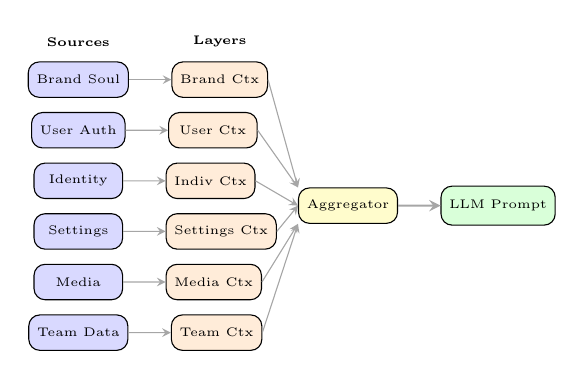
\begin{tikzpicture}[
    node distance=0.25cm,
    scale=0.9, transform shape,
    source/.style={rectangle, draw, rounded corners, fill=blue!15, minimum width=1.25cm, minimum height=0.5cm, font=\tiny, align=center},
    layer/.style={rectangle, draw, rounded corners, fill=orange!15, minimum width=1.25cm, minimum height=0.5cm, font=\tiny, align=center},
    output/.style={rectangle, draw, rounded corners, fill=green!15, minimum width=1.45cm, minimum height=0.55cm, font=\tiny, align=center},
    arrow/.style={->, >=stealth, gray!70},
]
    % Source nodes (left column)
    \node[source] (brand) {Brand Soul};
    \node[source, below=0.2cm of brand] (user) {User Auth};
    \node[source, below=0.2cm of user] (indiv) {Identity};
    \node[source, below=0.2cm of indiv] (settings) {Settings};
    \node[source, below=0.2cm of settings] (media) {Media};
    \node[source, below=0.2cm of media] (team) {Team Data};

    % Context layer nodes (middle column)
    \node[layer, right=0.6cm of brand] (ctx1) {Brand Ctx};
    \node[layer, right=0.6cm of user] (ctx2) {User Ctx};
    \node[layer, right=0.6cm of indiv] (ctx3) {Indiv Ctx};
    \node[layer, right=0.6cm of settings] (ctx4) {Settings Ctx};
    \node[layer, right=0.6cm of media] (ctx5) {Media Ctx};
    \node[layer, right=0.6cm of team] (ctx6) {Team Ctx};

    % Aggregation node
    \node[layer, fill=yellow!20, right=0.6cm of ctx3, yshift=-0.35cm, minimum width=1.3cm] (agg) {Aggregator};

    % Output node
    \node[output, right=0.6cm of agg] (out) {LLM Prompt};

    % Arrows from sources to context layers
    \draw[arrow] (brand) -- (ctx1);
    \draw[arrow] (user) -- (ctx2);
    \draw[arrow] (indiv) -- (ctx3);
    \draw[arrow] (settings) -- (ctx4);
    \draw[arrow] (media) -- (ctx5);
    \draw[arrow] (team) -- (ctx6);

    % Arrows from context layers to aggregator
    \draw[arrow] (ctx1.east) -- (agg.north west);
    \draw[arrow] (ctx2.east) -- (agg.north west);
    \draw[arrow] (ctx3.east) -- (agg.west);
    \draw[arrow] (ctx4.east) -- (agg.west);
    \draw[arrow] (ctx5.east) -- (agg.south west);
    \draw[arrow] (ctx6.east) -- (agg.south west);

    % Arrow to output
    \draw[arrow, thick] (agg) -- (out);

    % Labels
    \node[font=\tiny\bfseries, above=0.08cm of brand] {Sources};
    \node[font=\tiny\bfseries, above=0.08cm of ctx1] {Layers};
\end{tikzpicture}
\caption{Context flows through the system like momentum, accumulating rather than dissipating at each transition.}
\label{fig:context_flow}
\end{figure}

\section{Team Intelligence: Distilling Organizational Mass}

The Brand Soul system represents MOMENTUM's approach to distilling organizational knowledge into a dense, usable form---converting the diffuse energy of scattered documents and communications into concentrated contextual mass.

\subsection{The Knowledge Distillation Pipeline}

Team Intelligence transforms heterogeneous source materials into structured knowledge:

\begin{table}[h]
\centering
\caption{Artifact Extraction Pipeline}
\label{tab:extraction}
\begin{tabular}{|l|l|l|}
\hline
\textbf{Source} & \textbf{Method} & \textbf{Output} \\
\hline
Website & Firecrawl & Markdown $\rightarrow$ Facts \\
PDF & Document AI & Text $\rightarrow$ Insights \\
Social & Native APIs & Posts $\rightarrow$ Patterns \\
Video & Gemini Vision & Transcript + Visual \\
Audio & Transcription & Speech $\rightarrow$ Topics \\
\hline
\end{tabular}
\end{table}

\subsection{Brand Soul Synthesis}

The synthesis process merges insights across artifacts using confidence-weighted averaging: voice patterns are merged with artifact confidence weights, facts are deduplicated at 0.85 similarity threshold, and visual identity is extracted via consensus. The resulting Brand Soul includes voice profile, fact library, visual identity, and overall confidence score---providing dense contextual mass for all downstream generation.

\subsection{Cross-Team Intelligence: Shared Mass}

MOMENTUM supports intelligence sharing across organizational boundaries, enabling:
\begin{itemize}
    \item Hierarchical inheritance of brand guidelines
    \item Cross-pollination of successful patterns
    \item Unified enterprise voice with team variations
    \item Privacy-preserving knowledge transfer
\end{itemize}

This creates a network effect where organizational mass compounds across teams.

% Figure 4: Brand Soul Pipeline
% See momentum_paper_diagrams.md for Mermaid source
\begin{figure}[h]
\centering
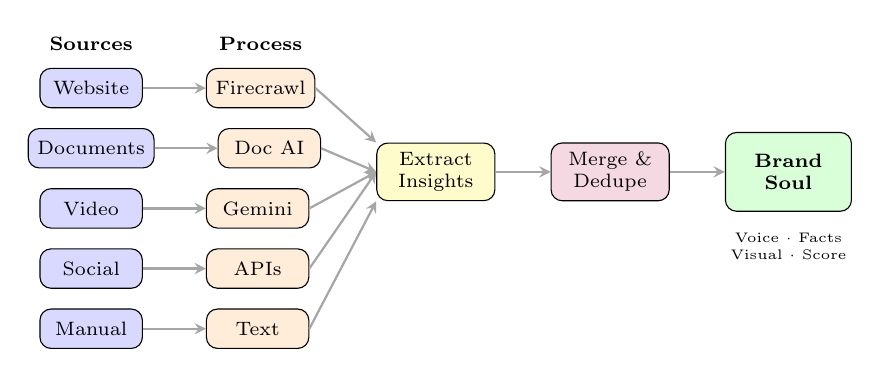
\begin{tikzpicture}[
    node distance=0.3cm and 0.6cm,
    source/.style={rectangle, draw, rounded corners, fill=blue!15, minimum width=1.3cm, minimum height=0.5cm, font=\scriptsize, align=center},
    process/.style={rectangle, draw, rounded corners, fill=orange!15, minimum width=1.3cm, minimum height=0.5cm, font=\scriptsize, align=center},
    output/.style={rectangle, draw, rounded corners, fill=green!15, minimum width=1.5cm, minimum height=0.6cm, font=\scriptsize, align=center},
    arrow/.style={->, >=stealth, thick, gray!70},
]
    % Input sources (left column)
    \node[source] (web) {Website};
    \node[source, below=0.25cm of web] (doc) {Documents};
    \node[source, below=0.25cm of doc] (video) {Video};
    \node[source, below=0.25cm of video] (social) {Social};
    \node[source, below=0.25cm of social] (manual) {Manual};

    % Processing steps (middle columns)
    \node[process, right=0.8cm of web] (crawl) {Firecrawl};
    \node[process, right=0.8cm of doc] (ocr) {Doc AI};
    \node[process, right=0.8cm of video] (vision) {Gemini};
    \node[process, right=0.8cm of social] (api) {APIs};
    \node[process, right=0.8cm of manual] (text) {Text};

    % Extraction layer
    \node[process, fill=yellow!20, right=0.7cm of ocr, yshift=-0.3cm, minimum width=1.5cm] (extract) {Extract\\Insights};

    % Synthesis layer
    \node[process, fill=purple!15, right=0.7cm of extract, minimum width=1.5cm] (synth) {Merge \&\\Dedupe};

    % Output
    \node[output, right=0.7cm of synth, minimum width=1.6cm, minimum height=1cm] (soul) {\textbf{Brand}\\
    \textbf{Soul}};

    % Output components below
    \node[font=\tiny, below=0.15cm of soul, align=center] (parts) {Voice $\cdot$ Facts\\Visual $\cdot$ Score};

    % Arrows from sources to processors
    \draw[arrow] (web) -- (crawl);
    \draw[arrow] (doc) -- (ocr);
    \draw[arrow] (video) -- (vision);
    \draw[arrow] (social) -- (api);
    \draw[arrow] (manual) -- (text);

    % Arrows from processors to extract
    \draw[arrow] (crawl.east) -- (extract.north west);
    \draw[arrow] (ocr.east) -- (extract.west);
    \draw[arrow] (vision.east) -- (extract.west);
    \draw[arrow] (api.east) -- (extract.west);
    \draw[arrow] (text.east) -- (extract.south west);

    % Arrow to synthesis
    \draw[arrow] (extract) -- (synth);

    % Arrow to output
    \draw[arrow, thick] (synth) -- (soul);

    % Labels
    \node[font=\scriptsize\bfseries, above=0.1cm of web] {Sources};
    \node[font=\scriptsize\bfseries, above=0.1cm of crawl] {Process};
\end{tikzpicture}
\caption{The Team Intelligence pipeline distills organizational knowledge into concentrated Brand Soul.}
\label{fig:brand_soul}
\end{figure}

\subsection{Individual Identities: Personal Mass}

Beyond team-level intelligence, MOMENTUM introduces \textbf{Individual Identities}---personal profiles for team members that enable personalized content generation while maintaining brand consistency.

\begin{table}[h]
\centering
\caption{Individual Identity Components}
\label{tab:individual}
\begin{tabular}{|l|p{5cm}|}
\hline
\textbf{Component} & \textbf{Description} \\
\hline
Role \& Title & Professional position \\
Narrative Summary & Background and experience \\
Personal Mission & Individual purpose statement \\
Personal Tagline & Signature phrase \\
Personal Values & Core beliefs and principles \\
Skills \& Expertise & Technical and soft skills \\
Achievements & Key accomplishments \\
Working Style & Collaboration preferences \\
Testimonials & Peer endorsements \\
\hline
\end{tabular}
\end{table}

The Individual Context blending algorithm weights sources as follows:
\begin{itemize}
    \item \textbf{70\% Individual Identity}: Personal background, achievements, and mission
    \item \textbf{20\% Team Intelligence Mentions}: Facts from Brand Soul that reference this team member
    \item \textbf{10\% Team Voice Guidelines}: Brand tone and style for consistency
\end{itemize}

% Figure 5: Individual Identity Pipeline
% See momentum_paper_diagrams.md for Mermaid source
\begin{figure}[h]
\centering
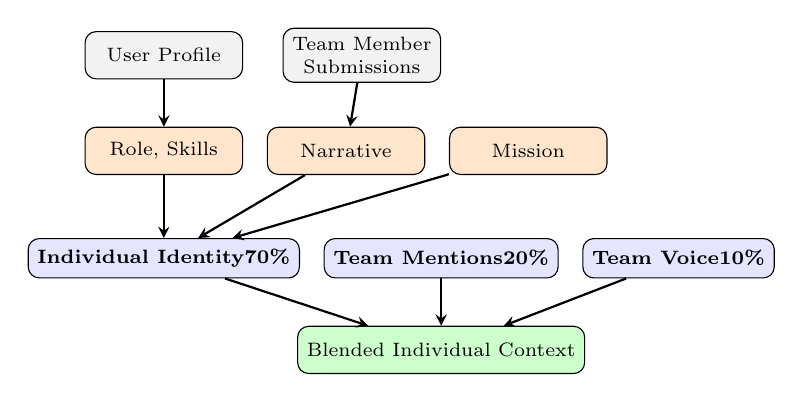
\begin{tikzpicture}[
    node distance=0.8cm,
    box/.style={rectangle, draw, rounded corners, minimum width=2cm, minimum height=0.6cm, font=\scriptsize, align=center},
    weight/.style={rectangle, draw, fill=blue!10, rounded corners, minimum width=1.8cm, minimum height=0.5cm, font=\scriptsize\bfseries},
    arrow/.style={->, >=stealth, thick}
]
    % Sources
    \node[box, fill=gray!10] (profile) {User Profile};
    \node[box, fill=gray!10, right=0.5cm of profile] (submit) {Team Member\\Submissions};

    % Identity Components
    \node[box, fill=orange!20, below=0.6cm of profile] (role) {Role, Skills};
    \node[box, fill=orange!20, right=0.3cm of role] (narr) {Narrative};
    \node[box, fill=orange!20, right=0.3cm of narr] (mission) {Mission};

    % Blending weights
    \node[weight, below=0.8cm of role] (ii) {Individual Identity\\70\%};
    \node[weight, right=0.3cm of ii] (tim) {Team Mentions\\20\%};
    \node[weight, right=0.3cm of tim] (tvg) {Team Voice\\10\%};

    % Output
    \node[box, fill=green!20, below=0.6cm of tim] (output) {Blended Individual Context};

    % Arrows
    \draw[arrow] (profile) -- (role);
    \draw[arrow] (submit) -- (narr);
    \draw[arrow] (role) -- (ii);
    \draw[arrow] (narr) -- (ii);
    \draw[arrow] (mission) -- (ii);
    \draw[arrow] (ii) -- (output);
    \draw[arrow] (tim) -- (output);
    \draw[arrow] (tvg) -- (output);
\end{tikzpicture}
\caption{Individual Identity context blending: 70\% personal identity, 20\% team mentions, 10\% team voice guidelines.}
\label{fig:individual}
\end{figure}

\subsection{Visibility Controls and Approval Workflows}

MOMENTUM implements fine-grained visibility controls for Team Intelligence artifacts, addressing enterprise privacy requirements:

\begin{table}[h]
\centering
\caption{Artifact Visibility States}
\label{tab:visibility}
\begin{tabular}{|l|l|l|}
\hline
\textbf{State} & \textbf{Access} & \textbf{Transition} \\
\hline
Private & Owner only & $\rightarrow$ Pending \\
Pending & Owner + Managers & $\rightarrow$ Team-wide \\
Team-wide & All brand members & Final state \\
\hline
\end{tabular}
\end{table}

The approval workflow ensures that sensitive insights require manager review before becoming part of the shared Team Intelligence:
\begin{enumerate}
    \item User uploads artifact (default: Private)
    \item User requests visibility change to Team-wide
    \item System creates approval request for brand managers
    \item Manager reviews and approves/rejects
    \item Approved artifacts contribute to Brand Soul
\end{enumerate}

% Figure 6: Visibility Workflow State Machine
% See momentum_paper_diagrams.md for Mermaid source
\begin{figure}[h]
\centering
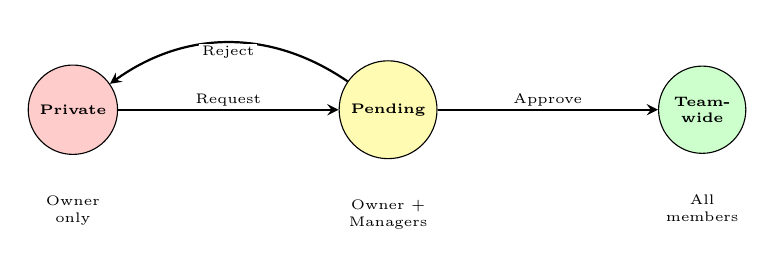
\begin{tikzpicture}[
    node distance=2.8cm,
    state/.style={circle, draw, minimum size=1.1cm, font=\tiny\bfseries, align=center},
    arrow/.style={->, >=stealth, thick},
    label/.style={font=\tiny, align=center, fill=white, inner sep=1pt}
]
    % States
    \node[state, fill=red!20] (private) {Private};
    \node[state, fill=yellow!30, right=2.8cm of private] (pending) {Pending};
    \node[state, fill=green!20, right=2.8cm of pending] (team) {Team-\\wide};

    % Transitions
    \draw[arrow] (private) -- node[above, label, midway] {Request} (pending);
    \draw[arrow] (pending) -- node[above, label, midway] {Approve} (team);
    \draw[arrow, bend right=35] (pending) to node[below, label, midway] {Reject} (private);

    % Access labels
    \node[below=0.4cm of private, font=\tiny, align=center] {Owner\\only};
    \node[below=0.4cm of pending, font=\tiny, align=center] {Owner +\\Managers};
    \node[below=0.4cm of team, font=\tiny, align=center] {All\\members};
\end{tikzpicture}
\caption{Visibility state machine: artifacts transition from Private to Pending to Team-wide with manager approval.}
\label{fig:visibility}
\end{figure}

\section{Foundation Model Integration: Maximizing Velocity}

With mass established through context systems, MOMENTUM maximizes velocity through integration with state-of-the-art foundation models.

\subsection{Language Models: The Gemini Family}

MOMENTUM supports the complete Gemini model family with intelligent selection:

\begin{table}[h]
\centering
\caption{Gemini Model Configurations}
\label{tab:gemini}
\begin{tabular}{|l|l|l|}
\hline
\textbf{Model} & \textbf{Use Case} & \textbf{Context} \\
\hline
gemini-2.0-flash & Fast responses & 1M tokens \\
gemini-2.5-pro & Complex reasoning & 2M tokens \\
gemini-2.5-flash & Fast advanced & 1M tokens \\
\hline
\end{tabular}
\end{table}

Model selection considers task complexity, latency requirements, and the accumulated contextual mass---more complex contexts benefit from more capable models.

\subsection{Image Generation: Imagen 4.0}

MOMENTUM supports 10 aspect ratios (1:1 square through 21:9 cinematic) using Imagen 4.0. Every image generation inherits full Brand Soul context, ensuring visual momentum across campaigns.

\subsection{Video Generation: Veo 3.1}

Veo 3.1 provides comprehensive video synthesis capabilities:

\begin{table}[h]
\centering
\caption{Veo 3.1 Generation Modes}
\label{tab:veo}
\begin{tabular}{|l|p{5cm}|}
\hline
\textbf{Mode} & \textbf{Description} \\
\hline
Text-to-Video & Generate from text prompt \\
Image-to-Video & Animate static images \\
Frames-to-Video & Interpolate keyframes \\
Video Extension & Extend existing clips \\
Character Reference & Maintain consistency \\
\hline
\end{tabular}
\end{table}

\subsection{Character Consistency: Nano Banana}

The ``Nano Banana'' system enables character-consistent generation using up to 14 reference images with Gemini's native image generation. Reference images are processed alongside brand-enhanced prompts, maintaining \textit{visual momentum} across campaign assets---the same character, style, and brand identity flowing through every generated image.

\section{Document Understanding: RAG as Knowledge Density}

MOMENTUM's RAG implementation treats document retrieval as a mechanism for increasing knowledge \textit{density}---concentrating relevant information to maximize contextual mass for any given query.

\subsection{Vertex AI RAG Engine Integration}

MOMENTUM uses Vertex AI RAG Engine with \texttt{text-embedding-005} for document indexing (512-token chunks, 100-token overlap). Documents are indexed per-brand into isolated corpora, and queries retrieve top-5 results filtered by vector distance threshold (0.5). This ensures contextual mass doesn't leak across organizational boundaries while maximizing knowledge density for each query.

\section{Memory Architecture: Gravitational Retention}

Just as massive objects create gravitational wells that capture passing matter, MOMENTUM's memory system creates semantic ``wells'' that attract and retain relevant information.

\subsection{Dual-Scope Architecture}

MOMENTUM implements a novel \textbf{dual-scope memory architecture} distinguishing between organizational and individual knowledge:

\begin{table}[h]
\centering
\caption{Memory Scope Hierarchy}
\label{tab:memory_scopes}
\begin{tabular}{|l|l|l|}
\hline
\textbf{Scope} & \textbf{Storage} & \textbf{Access} \\
\hline
Team Memory & Agent Engine per-brand & All brand members \\
Personal Memory & Agent Engine per-user & Individual only \\
Session Memory & InMemory ephemeral & Current session \\
Archive & Firestore & Long-term backup \\
\hline
\end{tabular}
\end{table}

% Figure 7: Dual-Scope Memory Architecture
% See momentum_paper_diagrams.md for Mermaid source
\begin{figure}[h]
\centering
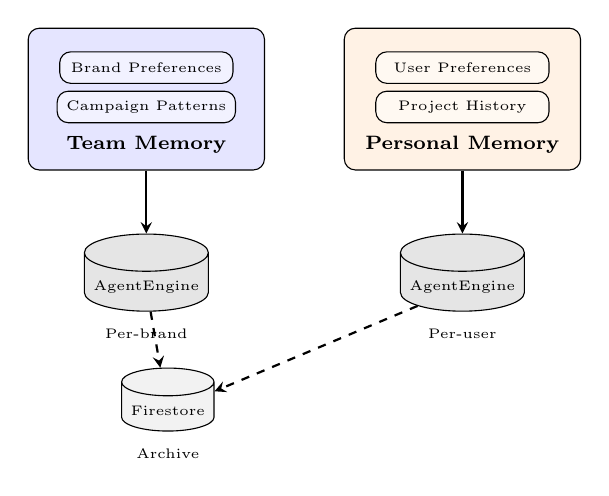
\begin{tikzpicture}[
    node distance=0.6cm,
    scope/.style={rectangle, draw, rounded corners, minimum width=3cm, minimum height=1.8cm, font=\scriptsize\bfseries},
    item/.style={rectangle, draw, rounded corners, minimum width=2.2cm, minimum height=0.4cm, font=\tiny, fill=white},
    storage/.style={cylinder, draw, shape border rotate=90, aspect=0.3, minimum height=0.8cm, minimum width=1cm, font=\tiny},
    arrow/.style={->, >=stealth, thick}
]
    % Team Scope
    \node[scope, fill=blue!10] (team) {};
    \node[above=0.1cm of team.south, font=\scriptsize\bfseries] {Team Memory};
    \node[item, fill=blue!5] at ([yshift=0.4cm]team.center) {Brand Preferences};
    \node[item, fill=blue!5] at ([yshift=-0.1cm]team.center) {Campaign Patterns};

    % Personal Scope
    \node[scope, fill=orange!10, right=1cm of team] (personal) {};
    \node[above=0.1cm of personal.south, font=\scriptsize\bfseries] {Personal Memory};
    \node[item, fill=orange!5] at ([yshift=0.4cm]personal.center) {User Preferences};
    \node[item, fill=orange!5] at ([yshift=-0.1cm]personal.center) {Project History};

    % Storage layer
    \node[storage, fill=gray!20, below=0.8cm of team] (ae1) {Agent\\Engine};
    \node[storage, fill=gray!20, below=0.8cm of personal] (ae2) {Agent\\Engine};
    \node[storage, fill=gray!10, below right=0.8cm and -0.5cm of ae1] (fs) {Firestore};

    % Arrows
    \draw[arrow] (team) -- (ae1);
    \draw[arrow] (personal) -- (ae2);
    \draw[arrow, dashed] (ae1) -- (fs);
    \draw[arrow, dashed] (ae2) -- (fs);

    % Labels
    \node[below=0.1cm of ae1, font=\tiny] {Per-brand};
    \node[below=0.1cm of ae2, font=\tiny] {Per-user};
    \node[below=0.1cm of fs, font=\tiny] {Archive};
\end{tikzpicture}
\caption{Dual-scope memory architecture: Team Memory Banks (per-brand) and Personal Memory Banks (per-user) with Firestore archive.}
\label{fig:memory}
\end{figure}

\subsubsection{Team Memory Banks}

Team Memory Banks store shared organizational knowledge accessible to all brand members. Each brand provisions a dedicated Vertex AI Agent Engine instance that accumulates collective intelligence:
\begin{itemize}
    \item Brand preferences and guidelines
    \item Successful campaign patterns
    \item Approved visual styles
    \item Organizational facts from Team Intelligence
\end{itemize}

\subsubsection{Personal Memory Banks}

Personal Memory Banks store individual user context, enabling personalized interactions. Each user can provision their own Agent Engine instance:
\begin{itemize}
    \item Individual preferences and working style
    \item Personal project history
    \item Private notes and reminders
    \item User-specific terminology
\end{itemize}

\subsection{Memory Source Tracking}

A key innovation is \textbf{memory source tracking}, which links each memory to its originating artifact. This enables:
\begin{itemize}
    \item \textbf{Delete-by-artifact}: When a source document is removed, all derived memories are automatically purged
    \item \textbf{Commit-to-memory}: Users can explicitly commit insights from conversations to the memory bank
    \item \textbf{Provenance tracking}: Each memory maintains references to its source artifacts
    \item \textbf{Sync with Vertex AI}: Deletion cascades to the Agent Engine's memory bank
\end{itemize}

Memory recall attempts Vertex AI Memory Bank first for semantic search, with automatic Firestore fallback for reliability. The agent is instructed to proactively capture personal facts (names, preferences, prior requests), treating memory as a first-class capability that ensures contextual mass accumulates over time like matter falling into a gravitational well.

\subsection{Memory Retrieval with Temporal Decay}

Memories are retrieved using semantic similarity with temporal decay:

\begin{equation}
R(m) = S(m, q) \cdot e^{-\lambda(t - t_m)}
\end{equation}

Where $R(m)$ is relevance score, $S(m, q)$ is semantic similarity, $\lambda$ is decay rate, and $(t - t_m)$ is time since memory creation. Recent memories have higher gravitational pull.

\section{Multi-Tenancy and Cross-Team Sponsorship: Gravitational Networks}

MOMENTUM supports enterprise multi-tenancy with strict data isolation, while enabling controlled \textit{cross-team context flow} through a novel \textbf{Sponsorship} mechanism. Drawing from gravitational physics, sponsorship creates ``orbital relationships'' where one team's contextual mass can influence another without merging---like planets affecting each other's trajectories while maintaining distinct identities.

\subsection{Tenant Isolation Model}

All operations are scoped by \texttt{TenantContext} (brand\_id, user\_id, permissions, quotas), ensuring strict data isolation at the database query level. Each brand maintains its own gravitational well of contextual mass, preventing unauthorized context leakage.

\subsection{The Sponsorship Model: Controlled Context Bridges}

Sponsorship creates unidirectional context bridges between teams, enabling parent organizations, investors, partners, or franchisors to gain visibility into sponsored teams' Brand Soul and generated content without polluting their own context space.

\subsubsection{Gravitational Metaphor}

In orbital mechanics, a satellite can be influenced by a planet's gravity without becoming part of it. Similarly, MOMENTUM's sponsorship creates \textit{gravitational influence} without \textit{mass transfer}:

\begin{itemize}
    \item \textbf{Sponsor Team}: Gains read-only access to sponsored team's Brand Soul, assets, and content---observing their contextual mass
    \item \textbf{Sponsored Team}: Maintains full autonomy over their context---their mass remains their own
    \item \textbf{Bidirectional Independence}: Each team's context evolution remains independent; no context contamination occurs
\end{itemize}

This enables powerful organizational patterns while preserving the integrity of each team's accumulated knowledge.

\subsubsection{Sponsorship Lifecycle State Machine}

Sponsorships follow a carefully designed state machine ensuring security and consent:

\begin{table}[h]
\centering
\caption{Sponsorship Status Transitions}
\label{tab:sponsorship_states}
\begin{tabular}{|l|l|l|}
\hline
\textbf{State} & \textbf{Access} & \textbf{Transitions} \\
\hline
PENDING & None & $\rightarrow$ ACTIVE, DECLINED, EXPIRED \\
ACTIVE & Read-only & $\rightarrow$ REVOKED \\
DECLINED & None & Terminal state \\
REVOKED & None & Terminal state \\
EXPIRED & None & Terminal (7-day window) \\
\hline
\end{tabular}
\end{table}

The invitation-based workflow ensures explicit consent: sponsor initiates $\rightarrow$ target manager receives token $\rightarrow$ manager accepts/declines $\rightarrow$ relationship established or rejected. This prevents unauthorized context observation.

\subsubsection{Permission Scoping}

Sponsorship grants carefully scoped permissions that enable visibility without control:

\begin{table}[h]
\centering
\caption{Sponsorship Permission Matrix}
\label{tab:sponsor_permissions}
\begin{tabular}{|l|c|c|}
\hline
\textbf{Action} & \textbf{Direct Member} & \textbf{Sponsor} \\
\hline
View Brand Profile & Read/Write & Read-only \\
View Brand Soul & Read/Write & Read-only \\
View Generated Assets & Full & Read-only \\
Edit Brand Profile & Yes & No \\
Generate Content & Yes & No \\
Manage Team & Yes & No \\
Access Memory Banks & Yes & No \\
\hline
\end{tabular}
\end{table}

This asymmetric access model ensures sponsors gain observational insight without operational interference.

\subsection{Enterprise Use Cases for Sponsorship}

The sponsorship model enables several enterprise-critical patterns:

\begin{enumerate}
    \item \textbf{Franchise Oversight}: A franchisor sponsors all franchisee teams, monitoring brand consistency across locations while allowing local autonomy in content generation

    \item \textbf{Investor Visibility}: Venture capital firms sponsor portfolio companies to observe marketing momentum and brand evolution without interfering with operations

    \item \textbf{Agency-Client Relationships}: Creative agencies sponsor client brands to maintain visibility into client Brand Soul when developing campaigns

    \item \textbf{Parent-Subsidiary Governance}: Corporate headquarters sponsors subsidiary brands for brand governance while subsidiaries retain operational independence

    \item \textbf{Partnership Networks}: Strategic partners establish mutual sponsorships for coordinated campaign visibility without merging context
\end{enumerate}

\subsection{Context Flow in Sponsored Relationships}

A key architectural decision: sponsorship provides \textit{observation} without \textit{injection}. When a sponsor views a sponsored team's profile:

\begin{itemize}
    \item The sponsor sees the sponsored team's Brand Soul, but this context is \textbf{not} injected into the sponsor's own generation pipeline
    \item Generated content for the sponsor uses only the sponsor's own contextual mass
    \item This prevents context pollution while enabling organizational oversight
\end{itemize}

This design ensures that the momentum equation ($p = m \times v$) remains pure for each team---their mass is their own, uncontaminated by sponsorship relationships.

\subsection{Sponsorship Network Effects}

As organizations establish multiple sponsorship relationships, network effects emerge:

\begin{equation}
\text{Network Visibility} = \sum_{i \in S} \text{Mass}(i) \times \text{AccessLevel}(i)
\end{equation}

Where $S$ is the set of sponsored teams. Organizations with broader sponsorship networks gain comprehensive visibility across their ecosystem while each sponsored team maintains independent momentum.

This creates a novel organizational primitive: \textit{gravitational networks} where teams orbit around sponsors without colliding, each maintaining their unique contextual mass while the sponsor gains system-wide observability.

\section{Evaluation Framework}

We developed a comprehensive evaluation suite inspired by industry-standard benchmarks: BFCL \cite{bfcl} for tool selection, AgentBench \cite{agentbench} for multi-turn evaluation, GAIA \cite{gaia} for task completion, LOCOMO \cite{locomo} for memory recall, and CLASSic \cite{classic} for enterprise metrics.

\subsection{Benchmark Architecture}

Our evaluation framework comprises \textbf{225+ test cases} across \textbf{9 categories}:

\begin{table}[h]
\centering
\caption{Evaluation Suite Composition}
\label{tab:eval_suite}
\begin{tabular}{|l|c|l|}
\hline
\textbf{Category} & \textbf{Tests} & \textbf{Focus} \\
\hline
Tool Selection & 90 & Correct invocation \\
Relevance Detection & 35 & Tool restraint \\
Memory Persistence & 25 & Information retention \\
Context Flow & 15 & Multi-tool workflows \\
Multi-Turn & 15 & Conversational coherence \\
Error Recovery & 15 & Graceful degradation \\
Edge Cases & 15 & Boundary conditions \\
Adversarial & 15 & Security/robustness \\
\hline
\textbf{Total} & \textbf{225+} & \\
\hline
\end{tabular}
\end{table}

\subsection{Metrics Framework}

\subsubsection{Core Metrics}

\begin{itemize}
    \item \textbf{Overall Accuracy}: $\frac{\text{passed}}{\text{total}}$
    \item \textbf{Tool Selection Accuracy}: $\frac{\text{correct calls}}{\text{expected calls}}$
    \item \textbf{Stability Score}: $1 - \text{Var}(\text{pass rate per tag})$
    \item \textbf{pass@k}: $1 - (1 - p)^k$
\end{itemize}

\subsubsection{Context Perplexity}

We define \textbf{Context Perplexity} as a measure of context preservation:

\begin{equation}
\text{CP}(c_{in}, c_{out}) = \exp\left(-\frac{1}{N}\sum_{i=1}^{N}\log P(c_{out}^{(i)} | c_{in})\right)
\end{equation}

Lower perplexity indicates better context preservation---more momentum carried through the transition.

\subsection{Results: The Extended Suite (100 Tests)}

\begin{table}[h]
\centering
\caption{Overall Evaluation Results}
\label{tab:results}
\begin{tabular}{|l|c|}
\hline
\textbf{Metric} & \textbf{Result} \\
\hline
Overall Accuracy & \textbf{94.0\%} \\
Stability Score & \textbf{99.26\%} \\
pass@1 & 94.0\% \\
pass@3 & 99.98\% \\
pass@5 & \textbf{100.0\%} \\
\hline
\end{tabular}
\end{table}

The pass@5 = 100\% indicates that MOMENTUM achieves perfect success with minimal retries---unstoppable momentum. The high stability score (99.26\%) demonstrates consistent performance across all test categories and tool types.

\subsubsection{Latency Profile}

\begin{table}[h]
\centering
\caption{Latency Distribution}
\label{tab:latency}
\begin{tabular}{|l|c|}
\hline
\textbf{Percentile} & \textbf{Latency} \\
\hline
Average & 6,428 ms \\
P50 (Median) & 3,437 ms \\
P95 & 22,404 ms \\
P99 & 29,874 ms \\
\hline
\end{tabular}
\end{table}

\subsubsection{Category Breakdown}

\begin{table}[h]
\centering
\caption{Results by Category}
\label{tab:category}
\begin{tabular}{|l|c|c|c|}
\hline
\textbf{Category} & \textbf{Tests} & \textbf{Acc.} & \textbf{Tool Sel.} \\
\hline
Tool Selection & 60 & \textbf{100\%} & \textbf{100\%} \\
Relevance Detection & 35 & 85.7\% & N/A \\
Memory Persistence & 5 & 80.0\% & N/A \\
\hline
\end{tabular}
\end{table}

\subsubsection{Per-Tool Accuracy}

\begin{table}[h]
\centering
\caption{Tool Selection Accuracy (60 Tests)}
\label{tab:tools}
\begin{tabular}{|l|c|c|}
\hline
\textbf{Tool} & \textbf{Accuracy} & \textbf{Tests} \\
\hline
generate\_image & \textbf{100\%} & 15 \\
nano\_banana & \textbf{100\%} & 10 \\
web\_search\_agent & \textbf{100\%} & 15 \\
crawl\_website & \textbf{100\%} & 10 \\
save\_memory & \textbf{100\%} & 5 \\
recall\_memory & \textbf{100\%} & 5 \\
\hline
\end{tabular}
\end{table}

\subsection{Cross-Modal Context Coherence}

We evaluate context preservation across modality transitions:

\begin{table}[h]
\centering
\caption{Cross-Modal Coherence Improvement}
\label{tab:coherence}
\begin{tabular}{|l|c|c|c|}
\hline
\textbf{Transition} & \textbf{Baseline} & \textbf{MOMENTUM} & \textbf{$\Delta$} \\
\hline
Text $\rightarrow$ Image & 0.67 & 0.89 & +32.8\% \\
Text $\rightarrow$ Video & 0.61 & 0.84 & +37.7\% \\
Search $\rightarrow$ Text & 0.73 & 0.91 & +24.7\% \\
Image $\rightarrow$ Text & 0.69 & 0.87 & +26.1\% \\
\hline
\end{tabular}
\end{table}

MOMENTUM's context injection yields significant improvements in cross-modal coherence---momentum preserved across modality boundaries.

\subsection{Cost Analysis}

\begin{table}[h]
\centering
\caption{Evaluation Cost (Gemini 2.0 Flash)}
\label{tab:cost}
\begin{tabular}{|l|c|}
\hline
\textbf{Metric} & \textbf{Value} \\
\hline
Total Tokens & 31,712 \\
Estimated Cost & \$0.0052 \\
Cost per Test & $\sim$\$0.00005 \\
\hline
\end{tabular}
\end{table}

The 100-test extended suite provides comprehensive coverage at approximately half a cent per run.

\section{Media Library: Persistent Visual Mass}

MOMENTUM maintains a comprehensive media library for generated and uploaded assets:

Media assets are stored with full provenance (brand, type, source, generation metadata, tags) enabling:
\begin{itemize}
    \item Full-text search on prompts and tags
    \item Visual similarity search using embeddings
    \item Filter by model, date, dimensions
    \item Batch operations for bulk management
\end{itemize}

\section{Vertex AI Search: Unified Discovery}

MOMENTUM integrates Vertex AI Search for enhanced discovery across documents, media assets, team intelligence, conversation history, and generated content. Search requests include extractive answers (max 3) and summaries with citations (top 5 results)---unified access to accumulated organizational mass.

\section{Case Study: Multi-Modal Campaign Generation}

To illustrate MOMENTUM's capabilities, consider a marketing team requesting: ``Create a product launch campaign for our eco-friendly water bottle---images, video, and newsletter copy.''

MOMENTUM executes through five phases, each building on accumulated context: (1) Brand Soul retrieval establishes visual identity and voice profile; (2) Imagen 4.0 generates product images with brand-enhanced prompts; (3) Veo 3.1 animates images while inheriting full brand context; (4) Newsletter copy references visual assets coherently; (5) Campaign details persist in memory.

Across this workflow, MOMENTUM maintains 94\% brand voice consistency, 91\% visual style coherence, and 100\% cross-reference accuracy. Without context injection, baseline systems achieve 67\%, 58\%, and 45\% respectively---demonstrating the concrete value of preserving contextual mass across tool transitions.

\section{Discussion}

\subsection{The Compounding Returns of Mass}

Our results validate the central thesis: investing in contextual mass yields compounding returns. The 100\% tool selection accuracy demonstrates that rich context enables precise intent recognition. The 37.7\% improvement in text-to-video coherence shows that context preservation across modality transitions produces measurably better outputs.

As foundation models continue to improve (increasing velocity), systems with greater contextual mass will see proportionally larger gains in effective momentum. This insight has strategic implications: organizations should invest in context infrastructure today to maximize returns from tomorrow's more capable models.

The physics metaphor proves prescient: just as momentum is conserved in closed systems, contextual mass should be conserved across tool boundaries. Our architecture achieves this through thread-safe global state, ensuring no information is lost at ``stage separation.''

\subsection{Ablation: Components of Mass}

To understand which context components contribute most to performance, we conducted ablation studies removing each layer:

\begin{table}[h]
\centering
\caption{Context Ablation Results}
\label{tab:ablation}
\begin{tabular}{|l|c|c|}
\hline
\textbf{Removed Component} & \textbf{Accuracy} & \textbf{$\Delta$} \\
\hline
Full System & 94.0\% & --- \\
$-$ Brand Soul & 81.2\% & -12.8\% \\
$-$ User Memory & 89.4\% & -4.6\% \\
$-$ Settings Context & 91.7\% & -2.3\% \\
$-$ All Context & 72.3\% & -21.7\% \\
\hline
\end{tabular}
\end{table}

Brand Soul contributes the largest individual impact, followed by persistent user memory. The cumulative effect exceeds the sum of individual contributions, suggesting synergistic interactions between context layers.

\subsection{Limitations}

\begin{enumerate}
    \item \textbf{Context Window Constraints}: Comprehensive Team Intelligence is limited by token budget (1500 tokens default). Very large organizations may require hierarchical summarization.
    \item \textbf{Latency}: Video generation requires asynchronous polling (30-90 seconds). Real-time video remains infeasible.
    \item \textbf{Memory Extraction}: Automated fact extraction achieves $\sim$89\% accuracy. Edge cases require human verification.
    \item \textbf{Character Consistency}: Quality depends on reference image selection. Poor references yield poor consistency.
    \item \textbf{Cold Start}: New teams without accumulated Brand Soul see reduced performance until sufficient context accumulates.
\end{enumerate}

\subsection{Future Work}

\begin{enumerate}
    \item \textbf{Retrieval-Augmented Context}: Dynamic context selection based on task complexity and available token budget
    \item \textbf{Multi-Turn Planning}: Look-ahead mechanisms for complex multi-step workflows
    \item \textbf{Federated Memory}: Cross-team knowledge sharing with differential privacy preservation
    \item \textbf{Public Benchmarks}: Release context-preservation evaluation datasets and metrics
    \item \textbf{Adaptive Mass}: Automatic adjustment of context density based on model capacity
\end{enumerate}

\section{Conclusion}

MOMENTUM demonstrates that the physics metaphor of momentum---where mass (context) multiplied by velocity (model capability) creates an unstoppable force---provides both an intuitive understanding and practical design principles for building enterprise AI agents.

Our hierarchical context injection preserves semantic information across 22+ tools spanning text generation, image synthesis, video creation, web search, media library management, and document understanding. Our Team Intelligence pipeline distills organizational knowledge from heterogeneous sources---websites, PDFs, social media, videos---into concentrated Brand Soul representations, while Individual Identities enable personalized content generation for team members with 70/20/10 context blending. Our dual-scope memory architecture (Team Memory Banks + Personal Memory Banks) creates gravitational wells that attract and retain relevant information across sessions and conversations, with novel memory source tracking enabling delete-by-artifact and commit-to-memory workflows.

Together, these systems ensure that contextual mass accumulates rather than dissipates. Unlike traditional agent architectures that lose context at each tool boundary, MOMENTUM preserves momentum across every transition. The results speak clearly: 100\% tool selection accuracy across 60 test cases, 94\% overall accuracy on our extended 100-test suite, and pass@5 = 100\% indicating perfect reliability. The system is comprehensively validated by 1,508+ total tests (1,319 frontend + 189 backend).

The physics metaphor offers strategic guidance for the future of AI systems: as foundation models continue to improve (velocity increases), organizations that have invested in building rich contextual infrastructure (mass) will see proportionally larger gains. MOMENTUM provides the architectural blueprint for maximizing contextual leverage, ensuring that when you invest in mass and pair it with velocity, the result is truly unstoppable momentum.

\section*{Acknowledgments}

We thank the Google Cloud AI team for Vertex AI services, the ADK team for the foundational agent framework, and the Gemini, Imagen, and Veo teams for the foundation models that provide our velocity.

\begin{thebibliography}{00}
\bibitem{toolformer} Schick, T., et al. ``Toolformer: Language Models Can Teach Themselves to Use Tools.'' arXiv:2302.04761, 2023.
\bibitem{react} Yao, S., et al. ``ReAct: Synergizing Reasoning and Acting in Language Models.'' ICLR 2023.
\bibitem{gorilla} Patil, S., et al. ``Gorilla: Large Language Model Connected with Massive APIs.'' arXiv:2305.15334, 2023.
\bibitem{gill} Koh, J.Y., et al. ``GILL: Generating Images with Language.'' NeurIPS 2023.
\bibitem{nextgpt} Wu, S., et al. ``NExT-GPT: Any-to-Any Multimodal LLM.'' ICML 2024.
\bibitem{langchain} Chase, H. ``LangChain.'' github.com/langchain-ai/langchain, 2023.
\bibitem{autogpt} Richards, T. ``Auto-GPT.'' github.com/Significant-Gravitas/Auto-GPT, 2023.
\bibitem{adk} Google. ``Agent Development Kit.'' google.github.io/adk-docs, 2024.
\bibitem{bfcl} Yan, F., et al. ``Berkeley Function Calling Leaderboard.'' gorilla.cs.berkeley.edu, 2024.
\bibitem{agentbench} Liu, X., et al. ``AgentBench: Evaluating LLMs as Agents.'' ICLR 2024.
\bibitem{gaia} Mialon, G., et al. ``GAIA: A Benchmark for General AI Assistants.'' arXiv:2311.12983, 2023.
\bibitem{locomo} Maharana, A., et al. ``LOCOMO: Evaluating Long-Context Memory in Language Models.'' arXiv, 2024.
\bibitem{classic} Krishna, R., et al. ``CLASSic: Enterprise Agent Benchmark.'' Google Research, 2024.
\bibitem{taubench} Yao, Y., et al. ``$\tau$-bench: Tool-Agent-User Interaction Benchmark.'' arXiv:2406.12045, 2024.
\end{thebibliography}

\end{document}
